\documentclass[12pt]{article}

\usepackage[paperwidth=8.27in, paperheight=11.69in, left=2.0cm, top=2.0cm, right=2.0cm, bottom=1.5cm]{geometry}
\usepackage{times, graphicx, amsmath, bm, units}
\usepackage{url, multirow, color}
\usepackage[hidelinks]{hyperref}
\usepackage[font=small,labelfont=bf]{caption}

%for highlighting in math mode:
\usepackage{xcolor}
\newcommand{\highlight}[1]{%
  \colorbox{yellow!75}{$\displaystyle#1$}}


\renewcommand{\floatpagefraction}{0.95}
\renewcommand{\textfraction}{0}
\renewcommand{\topfraction}{1}
\renewcommand{\bottomfraction}{1}


\begin{document}
\thispagestyle{empty}

\title{Implementation of a stable numerical scheme to solve the 1D diffusion equation with variable coefficients and source terms subject to Neumann boundary conditions}
\author{Jake Aylmer}
\maketitle

%%%%%%%%%%%%%%%%%%%%%%%%%%%%%%%%%%%%%%%%%%%%%%%%%%%%%%%%%%%%%%%%%%%%%%%%%%%%%%%%
\section{Problem statement}

The one-dimensional diffusion equation for tracer $q(x,t)$, defined on $0<x<L$ and $t\geq 0$, with source $S(x,t)$ and diffusivity $k(x)$ is given by
\begin{equation}\label{eq:diffusionequation}
\frac{\partial q}{\partial t} - \frac{\partial}{\partial x}\left[k(x)\frac{\partial q}{\partial x}\right] = S(x,t),
\end{equation}
which is subject to Neumann boundary conditions (zero flux of $q$ at the boundaries)
\begin{equation}\label{eq:boundaryconditions}
k(0)\frac{\partial q}{\partial x}\Bigr|_{x=0} = k(L)\frac{\partial q}{\partial x}\Bigr|_{x=L}= 0
\end{equation}
and specified initial conditions
\begin{equation}\label{eq:initialconditions}
q(x,0) = q_0(x).
\end{equation}

%%%%%%%%%%%%%%%%%%%%%%%%%%%%%%%%%%%%%%%%%%%%%%%%%%%%%%%%%%%%%%%%%%%%%%%%%%%%%%%%
\section{Analytic solution for a limiting case}

Equation (\ref{eq:diffusionequation}) can be solved analytically in the limit of no sources or sinks ($S(x,t)=0$) and constant diffusivity $k(x)=k_0$. This is derived by using the method of separation of variables and expressing the general solution as an infinite sum of normal modes with coefficients found using Fourier analysis. The final result is given here and can be used as a test for the numerical solution to the full diffusion equation (\ref{eq:diffusionequation}). The solution to
\begin{equation}\label{eq:simplifieddiffusionequation}
\frac{\partial q}{\partial t} = k_0\frac{\partial^2q}{\partial x^2}
\end{equation}
is given by
\begin{equation}\label{eq:analyticsolution}
q(x,t) = a_0 + \sum_{n=1}^\infty a_n \mathrm{exp}\left(-k_0\left(\frac{n\pi}{L}\right)^2t\right)\cos\left(\frac{n\pi}{L}x\right)
\end{equation}
where the coefficients $a_n$ are those found in the cosine series expansion of the initial conditions $q_0(x)$:
\begin{equation}\label{eq:a0}
a_0 = \frac{1}{L}\int_0^Lq_0(x)\mathrm{d}x
\end{equation}
\begin{equation}\label{eq:an}
a_n = \frac{2}{L}\int_0^Lq_0(x)\cos\left(\frac{n\pi}{L}x\right)\mathrm{d}x\hspace{5mm} n\geq 1.
\end{equation}

\subsection{Specific case for testing}
Choose initial conditions
\begin{equation}\label{eq:initialconditionsexample}
q_0(x) = q_\mathrm{max}x(L-x)
\end{equation}
where $q_\mathrm{max}$ is a constant corresponding to the maximum of $q_0$ occuring at $x=L/2$. This allows for the $a_n$ to be easily solved from equation (\ref{eq:an}):
\begin{equation}
a_0 = \frac{q_\mathrm{max}L^2}{6},\hspace{5mm} a_n = -2q_\mathrm{max}\left(\frac{L}{n\pi}\right)^2\left[1+\left(-1\right)^n\right]\hspace{5mm} n \geq 1
\end{equation}
(i.e. $a_n=0$ if $n$ is odd). The solution is thus
\begin{equation}\label{eq:specificanalyticsolution}
q(x,t) = \frac{q_\mathrm{max}L^2}{6} -\frac{4q_\mathrm{max}L^2}{\pi^2}\sum_{n\ \mathrm{even}}\frac{1}{n^2}\mathrm{exp}\left(-k_0\left(\frac{n\pi}{L}\right)^2t\right)\cos\left(\frac{n\pi}{L}x\right).
\end{equation}
In the limit $t\rightarrow\infty$, $q(x,t)\rightarrow q_\mathrm{max}L^2/6$.


%%%%%%%%%%%%%%%%%%%%%%%%%%%%%%%%%%%%%%%%%%%%%%%%%%%%%%%%%%%%%%%%%%%%%%%%%%%%%%%%
\section{Implementation of numerical solution}
The numerical scheme is summarised here but not derived.\footnote{See, for example, \color{blue}\underline{\href{http://www.csc.kth.se/utbildning/kth/kurser/DN2255/ndiff13/Lecture3.pdf}{\smash{http://www.csc.kth.se/utbildning/kth/kurser/DN2255/ndiff13/Lecture3.pdf}}}\color{black}} The $x$ domain is discretised into $N$ grid cells, labelled from $j=0$ to $j=N-1$, each of width $h = L/N$. $q$ and $S$ are then defined at the grid-cell centres, and expressed as $N$-element vectors $\mathbf{q}=[q(x_0),...,q(x_j),...,q(x_{N-1})]^\mathrm{T}$ and $\mathbf{S}$ defined similarly, where $x_j\equiv(j+\nicefrac{1}{2})h$.\footnote{Technically, $q(x_j)$ should be written as, say, $\tilde{q}(x_j)$, to indicate that it is the integral average over the grid cell, but this subtlety is ignored for simplicity} See figure (\ref{fig:gridschematic}).
\begin{figure}[h]
\centering
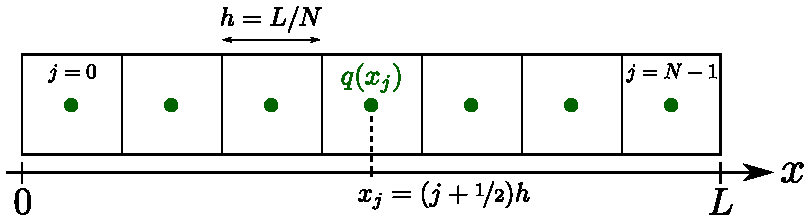
\includegraphics[width=0.8\linewidth]{grid_schematic.pdf}
\caption{Schematic showing how the domain is discretised into $N$ cells of equal widths $h$. $q$ (green) is calculated at grid cell centres (as is $S$).}
\label{fig:gridschematic}
\end{figure}

\noindent
Equation (\ref{eq:diffusionequation}) is re-written in the semi-discretised form
\begin{equation}\label{eq:semidiscrete}
\frac{d\mathbf{q}}{dt} = \mathsf{A}\mathbf{q} + \mathbf{S}
\end{equation}
where the $(N\times N)$ matrix $\mathsf{A}$ takes the place of the operator $\partial_x(k(x)\partial_x)$ in equation (\ref{eq:diffusionequation}). $\mathsf{A}$ accounts for the boundary conditions of the problem: \textit{here and in the code only Neumann boundary conditions are used}. The result is as follows for elements $\mathsf{A}_{ij}$ where $i$ refers to the row index and $j$ the column index, and $k_j\equiv k(x_j)=k((j+\nicefrac{1}{2})h)$. For $i\neq 0$, $i\neq N-1$:
\begin{equation}\label{eq:matrixelements}
h^2\mathsf{A}_{ij} = \begin{cases}
    -(k_{j+\nicefrac{1}{2}}+k_{j-\nicefrac{1}{2}}) & i=j \\
    k_{j\pm\nicefrac{1}{2}} & i=j\pm1, \\
    \end{cases}
\end{equation}

\clearpage
\noindent
and for the boundaries:
\begin{equation}
\nonumber
h^2\mathsf{A}_{00} = -k_{\nicefrac{1}{2}}
\end{equation}
\begin{equation}
\nonumber
h^2\mathsf{A}_{01} = k_{\nicefrac{1}{2}}
\end{equation}
\begin{equation}
\nonumber
h^2\mathsf{A}_{(N-1),(N-2)} = k_{N-\nicefrac{3}{2}}
\end{equation}
\begin{equation}\label{eq:matrixelementsboundaries}
h^2\mathsf{A}_{(N-1),(N-1)} = -k_{N-\nicefrac{3}{2}}.
\end{equation}
Equation (\ref{eq:semidiscrete}) is then discretised in time (to give the fully-discrete scheme) using the $\theta$-method. $\theta$ is a parameter between $0$ and $1$ which determines whether the scheme is explicit or implicit and first or second order accurate. This results in
\begin{equation}\label{eq:numericalscheme}
\mathbf{q}^{n+1}=\left[\mathsf{I}-\theta\Delta t\mathsf{A}\right]^{-1}\left[\left(\mathsf{I}+(1-\theta)\Delta t\mathsf{A}\right)\mathbf{q}^n + \Delta t\mathbf{S}_\theta^n\right]
\end{equation}
where $\Delta t$ is the time-step, $\mathsf{I}$ is the $N$-dimensional identity matrix, superscript $n$ refers to the time level and
\begin{equation}\label{eq:Stheta}
\mathbf{S}_\theta^n = \theta\mathbf{S}^{n+1}+(1-\theta)\mathbf{S}^n.
\end{equation}
The value of $\theta$ can be set in the code and corresponds to:

\begin{center}
\begin{tabular}{ cccc }
$\theta$ & Name & Type & Accuracy \\
\hline
$0$ & Forward-Euler & Explicit & $1^\mathrm{st}$ order \\
$\nicefrac{1}{2}$ & Crank-Nicolson & Implicit & $2^\mathrm{nd}$ order \\
$1$ & Backward-Euler & Implicit & $1^\mathrm{st}$ order \\
\end{tabular}
\end{center}

An example of the numerical scheme being used to solve the diffusion equation (\ref{eq:simplifieddiffusionequation}) with $k_0=2.5\times 10^{-3}$ m$^2$s$^{-1}$, $L=2.0$ m and initial conditions (\ref{eq:initialconditionsexample}) with $q_\mathrm{max}=4$ is shown in figure (\ref{fig:example}). This was carried out on a grid with $N=20$ ($\Rightarrow h=0.1$ m) and using time-step $\Delta t=5$ s, for $6$ time steps. The Forward Euler method ($\theta=0$) is severely time-step restricted and is not plotted.

\begin{figure}[b]
\centering
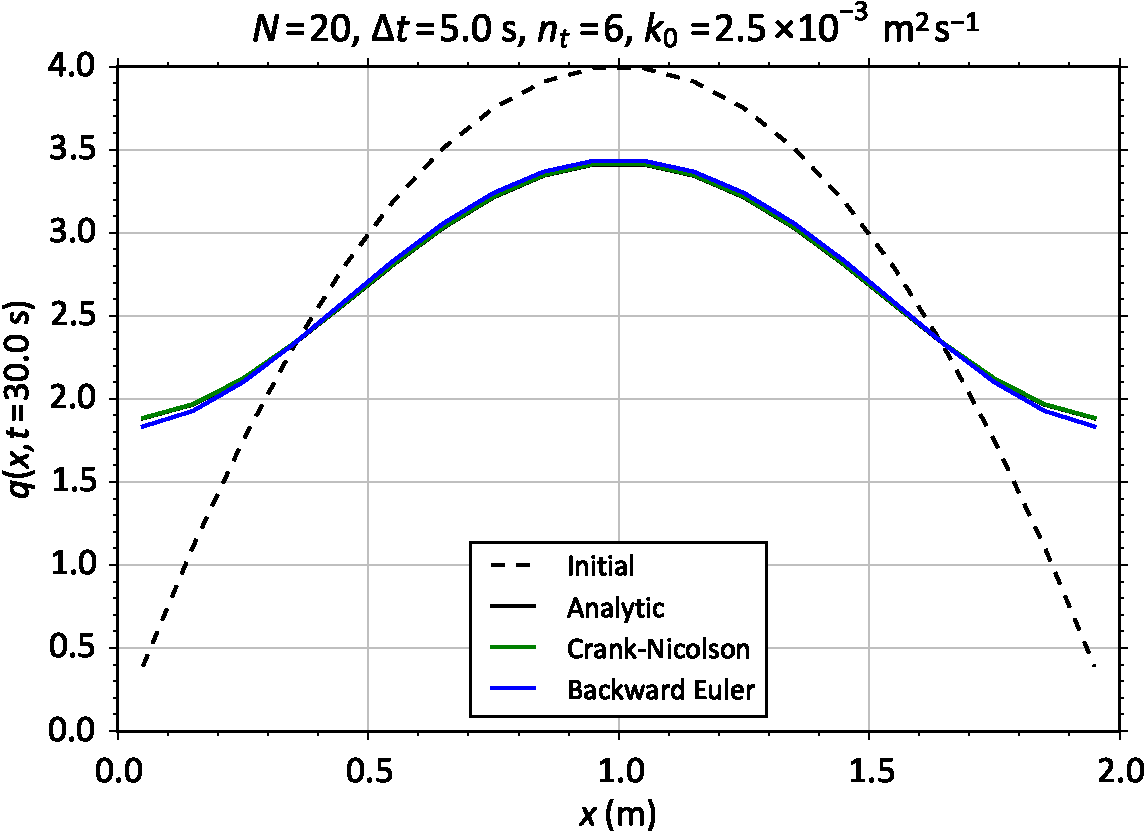
\includegraphics[width=0.7\linewidth]{example_plot.pdf}
\caption{Example solution of the simplified diffusion equation (\ref{eq:simplifieddiffusionequation}) with initial conditions (\ref{eq:initialconditionsexample}) (dashed-line), $L=2.0$ m, $q_\mathrm{max}=4.0$ and other parameters as listed at the top of the figure. The analytic solution (\ref{eq:specificanalyticsolution}) is plotted (black) but is obscured by the numerical solutions, which were calculated using the scheme implementation (\ref{eq:numericalscheme})-(\ref{eq:Stheta}) setting $\mathbf{S}=0$ and $k(x)=k_0$. The Crank-Nicolson solution (green) is more accurate than the Backward-Euler solution (blue) as expected (this can be seen by zooming in on the solutions). The Forward-Euler solution is not plotted because it requires a significantly smaller time-step for numerical stability.}
\label{fig:example}
\end{figure} 




\end{document}